\chapter{Méthodes de représentation et d'analyse de l'architecture CxSOM}
\graphicspath{{03-Representation/}}

\minitoc
\section{Représentation des cartes de Kohonen}

\subsection{Représentations et indicateurs classique des cartes de Kohonen}

Les cartes de Kohonen sont particulièrement associées à une facilité de représentation et de visualisation. En effet, leur nombre réduit de prototypes et leur aspect topologique permet d'en tracer une représentation visuelle interprétable.
La manière la plus utilisée de représenter une carte de Kohonen est de tracer les poids de ses prototypes, disposés dans le graphe qu'est la carte. En fonction des dimensions des entrées, cette représentation prennent plusieurs formes. Deux exemples courants de représentation sont les suivants: 
\begin{itemize}
\item Le graphe qu'est la carte de Kohonen est représenté dans l'espace de ses positions (la grille d'indices $(i,j)$, ou une ligne indexée par $i$. Sur chaque noeud est tracé le poids correspondant. C'est le cas sur l'exemple de gauche en figure~\ref{fig:representation} dans lequel les poids des prototypes, qui sont des imagettes, sont affichés en chaque point de la grille. Si la dimension d'un poids est trop grande pour être représentée graphiquement, il est également courant d'étiquetter chaque prototype et d'afficher ces étiquettes sur les noeuds de la carte, en tant que représentation.
\item Lorsque les données traitées sont des points deux ou trois dimensions, les poids des prototypes peuvent être directement tracés dans l'espace $\mathbb{R}^2$ ou $\mathbb{R}^3$. Ces poids sont alors reliés en fonction des positions des noeuds dans la carte, montrant ainsi la déformation de la carte dans l'espace d'entrée, c'est le cas sur l'exemple de droite en figure~\ref{fig:representation}.
\end{itemize}

\begin{figure}
\begin{minipage}{0.5\textwidth}
\centering
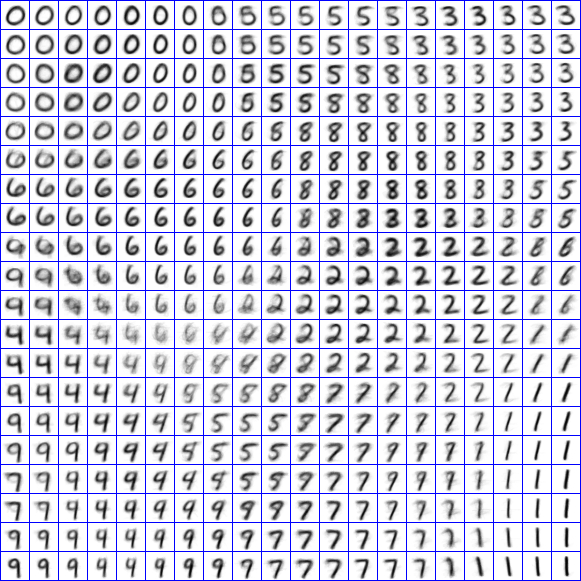
\includegraphics[width=0.5\textwidth]{digits.jpg}
\end{minipage}
\begin{minipage}{0.5\textwidth}
\centering
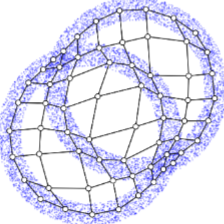
\includegraphics[width=0.5\textwidth]{points.png}
\end{minipage}
\label{fig:representation}
\caption{Représentations possible des poids d'une carte de Kohonen classiques, dans le cas d'entrées sous forme d'imagettes ou de points en deux dimensions.}
\end{figure}

\draft{Distortion d'une carte : une mesure de la différence moyenne des entrées par rapport à tous les centroïdes}

%
%On parle ici d'interprétation visuelle humaine. Pour l'oeil humain, cette facilité d'interprétation est limitée à un domaine d'utilisation: celui dans lequel les éléments qui nous intéressent sont les distances euclidiennes entre les données, ou plus généralement dans lequel la distance considérée pour la mise a jour des cartes possède un aspect graphique facilement interprétable. Essayez par exemple de vous représenter des distances dans un espace non-euclidien, ou des distances . Savoir quels points sont les plus proches nécessite alors un effort mental important et non une seule intuition; finalement la façon la plus simple de le savoir est de faire le calcul.
 
%La représentation d'une carte cherche à répondre à la question: "est-ce que la carte est bien dépliée sur toutes les données ? Est-ce qu'un prototype représente correctement une donnée ?". Y répondre en visualisant ses prototypes revient au processus intellectuel suivant: l'observateur imagine une donnée, par exemple une imagette d'un chiffre à main levée, et reproduit le processus de sélection du BMU qui a eu lieu lors de l'apprentissage de la carte pour trouver le poids qui lui correspond le mieux. Via ce processus mental, on est capable d'évaluer si une carte est dépliée sur les données. 
%Imaginons à présent que les distances considérées entre les éléments d'une carte ne soient plus euclidiennes: cette évaluation du dépliement de la carte repose maintenant sur soit une capacité d'abstraction phénoménale de l'observateur. Un exemple est donné en figure~\ref{fig:non_eucl}: l'observateur humain visualise un distance euclidienne($L^2$), éventuellement une distance de Manhattan. Mais si les distance sont calculées autrement, l'observateur préferera les nombres à la représentaiton graphique, ou une représentation dans un espace qui lui est familier. La représentation de la carte doit ainsi être adaptée au processus d'organisation.
%% Ajouter ref : mesures usuelles des cartes de Kohonen ? Pourquoi ne les utilise ton pas ?
%
% 
%Ainsi, pour représenter un algorithme d'apprentissage non-supervisé et en particulier une carte de Kohonen, on doit d'abord bien poser ce qu'on cherche à évaluer : l'entrée de l'algorithme est bien définie, sa sortie correspond à tous les éléments présents dans la carte. Un choix de représentation est donc à réaliser. Ensuite, cette représentation doit être adaptée aux règles de calcul de l'algorithme, ici de l'espace de la carte. 


\subsection{Que cherche t-on à représenter dans CxSOM ?}

Nous présenterons dans ce chapitre les choix de tracés et représentation des cartes auto-organisatrices utilisées dans une architecture CxSOM.
Les exemples de représentations présentés tout au long de ce chapitre s'appuient sur l'expérience illustrée en figure~\ref{fig:exp}: nous étudions une architecture composée de deux cartes en une dimension, chacune étant connectée à sa voisine. Les entrées des cartes sont $X$ et $Y$, les coordonnées d'un cercle. Ces deux modalités sont dépendantes: pour une valeur de $X$, deux valeurs sont possible pour $Y$, et symmétriquement.

\begin{figure}
\begin{minipage}{0.4\textwidth}
\centering
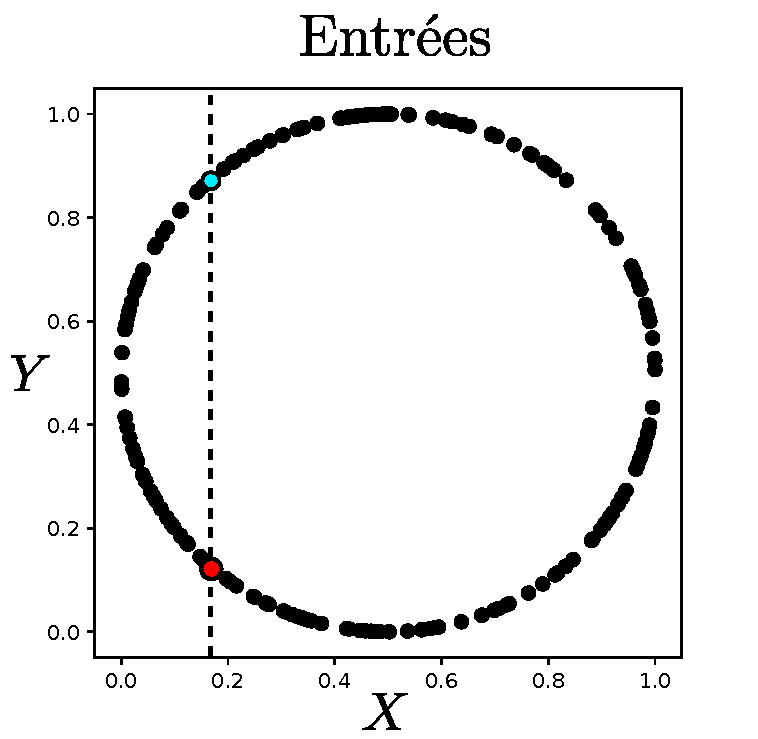
\includegraphics[width=0.8\textwidth]{2som_inp_noinformation}
\end{minipage}
\begin{minipage}{0.6\textwidth}
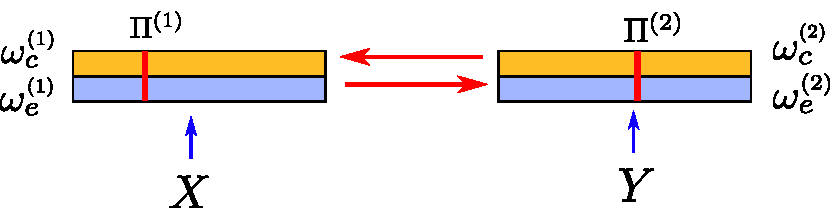
\includegraphics[width=\textwidth]{2som_archi}
\end{minipage}
\label{fig:exp}
\caption{Disposition des entrée, sous forme de cercle, à gauche, et architecture de deux cartes en une dimension étudiée et représentée dans ce chapitre.}
\end{figure}

La figure~\ref{fig:weights} présente le tracé des poids des deux cartes de l'exemple après apprentissage. Ce tracé permet de conclure que les cartes sont bien dépliées et ont transcrit une continuité dans les ensemble d'entrée. Cependant, il manque l'information nécessaire pour comprendre les mécanismes impliqués dans l'apprentissage de ces cartes. En effet, le choix du BMU dépend de plusieurs entrées et du processus de relaxation. La représentation des poids seuls ne permet pas de comprendre quels seront les BMUs de chaque carte pour une entrée donnée. 


La représentation visuelle d'une cartes d'une architecture est limitée par la dimension des entrées et la dimension des cartes. Dans l'exemple, les entrées et les cartes sont en une dimension, représenter leurs poids est donc réalisable; en plus grande dimension, il sera nécessaire d'utiliser une représentation telle que celle décrite en figure~\ref{fig:representation}. Le nombre de connexions contextuelles limitera alors également la lecture d'un tracé. Cette difficulté de représentation soulève la nécessité de définir des valeurs indicatrices du fonctionnement de la carte, calculables en grande dimension.

\begin{figure}
\centering
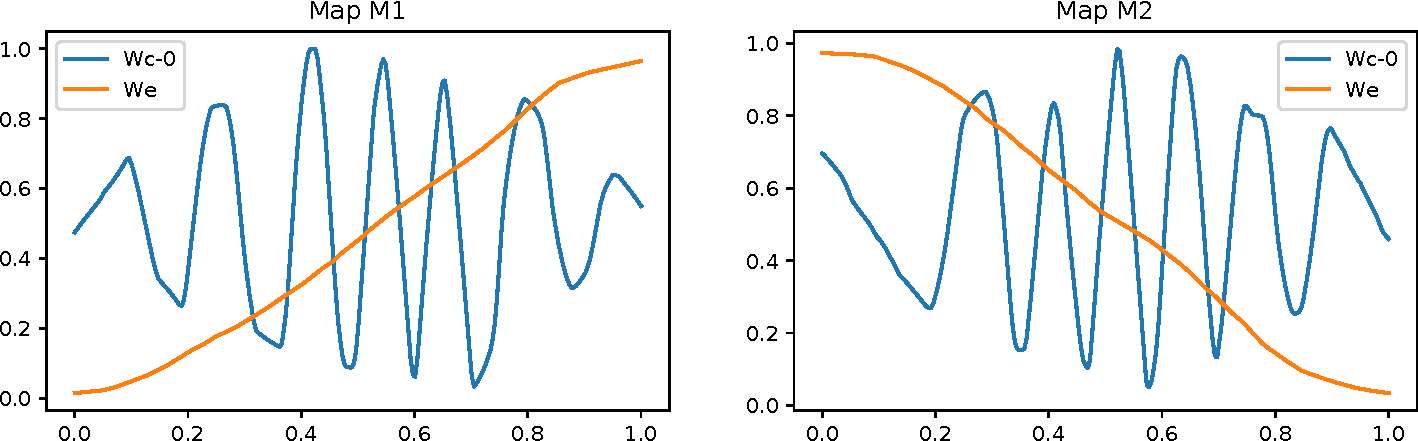
\includegraphics[width=0.9\textwidth]{weights_cercle1.pdf}
\label{fig:weights}
\caption{Représentation des valeurs des poids d'une carte au sein de CxSOM après apprentissage. La seule représentation de ces poids ne suffit pas à savoir comment la carte se comporte.}
\end{figure}

Ensuite, CxSOM s'intéresse à la communication entre cartes et la représentation des dépendances entre modalités. Représenter les cartes une à une laisse donc de coté leur connexion. Il est donc nécessaire de trouver un moyen de représenter l'architecture comme un tout. La représentation cherchera notamment à montrer comment l'architecture de cartes est capable d'apprendre les relations entre les entrées multimodales.

Ce chapitre questionne donc la façon de représenter une carte au sein d'une architecture. Nous présenterons en premier lieu un formalisme décrivant les cartes et leurs entrées multimodales associées. A partir de ce formalisme, nous proposerons plusieurs représentations et indicateurs permettant de comprendre et représenter ce que calcule une architecture CxSOM sur les données d'entrées. Nous utiliserons ces représentations et indicateurs dans les chapitres suivants. 

\section{Formalisme: variables aléatoires}

Nous introduisons dans cette section un formalisme traitant les éléments des cartes et les entrées en tant que variables aléatoires. Ce formalisme a l'avantage de à la fois clarifier les représentations, et de permettre le développement d'indicateurs statistiques sur les cartes.

\subsection{Représentation des entrées}

Les observations multimodales que l'on cherche à apprendre par l'architecture de cartes sont notées ${\inpx\m{i}, i = 0 \cdots N}$ où $N$ est le nombre de modalités considérées. A chaque pas de temps, un vecteur $\mathbf{\inpx} = (\inpx\m{0}, \cdots , \inpx\m{N})$ est présenté à l'architecture. Il s'gait d'une réalisation de la variable jointe $\mathbf{X}$.

On s'intéressera particulièrement à l'apprentissage de relations entre entrées. Les variables $\inpx\m{i}$ ne sont donc pas des variables indépendantes. On choisit  de représenter cette dépendance par une autre variable aléatoire $U$. Cette variable est multidimensionnelle et choisie de façon à ce que chaque variable $\inpx\m{i}$ soit une fonction quelconque de la variable aléatoire $U$, et uniquement de cette variable.

\begin{equation}
\forall i, \inpx\m{i} = f\m{i}(U)
\label{eq:U}
\end{equation}

Il s'agit d'une réduction de dimension qui traduit l'existence d'un modèle reliant les observations.
Dans le cas d'exemple, $\mathbf{X} = (X,Y)$, les coordonnées cartésiennes des points du cercle est alors une vecteur aléatoire, dont les composantes sont les variables aléatoires $X,Y$. En définissant une variable $U$ à valeurs réelles, chaque point du du cercle peut maintenant s'écrire, selon l'équation paramétrique du cercle:
\begin{equation}
 \begin{cases}
     X = r  \cos(2\pi U)\\
     Y = r \sin(2 \pi U)
    \end{cases}\,.
\end{equation}

$U$ représente ici l'angle du point sur le cercle. $U$ est une variable cachée qui réduit la dimension du modèle. Et contient toute l'information sur l'échantillon. 
$U$ et $f\m{i}$ ne sont pas uniques. Elle sont choisies en fonction de ce qu'on cherche à traduire dans le modèle. Ainsi, pour le même ensemble de points sous forme de cercle, on pourrait aussi définir une variable $U$ en deux dimensions, une dimension à valeur réelles paramétrisant un demi cercle, l'autre à valeurs dans ${0,1}$ indiquant de quel coté de l'axe des abscisses on se situe. Ces paramétrisations sont exprimées en figure \ref{fig:U}.
Par contre, la plus petite dimension possible de $U$ dépend du degré de liberté du modèle. Si toutes les observations se situent sur une courbe de dimension 1, alors il existe une variable $U$ en une dimension satisfaisant l'équation~\ref{eq:U}. Si les observations se situent sur une surface de dimension 2, alors, $U$ sera en deux dimensions, et ainsi de suite. 
Les exemples donnés sont scalaires, mais cette représentation générale à n'importe quel dimension et nombre d'entrées.

\begin{figure}
\begin{minipage}{0.5\textwidth}
\centering
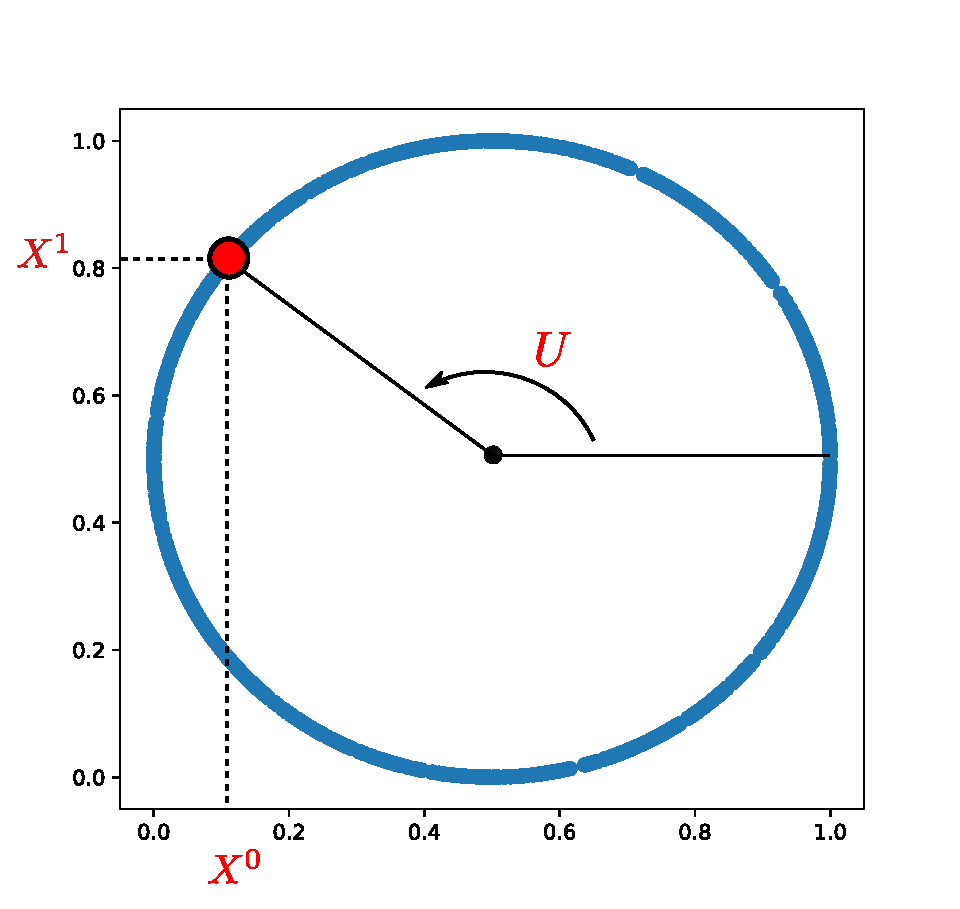
\includegraphics[width=0.6\textwidth]{cercle.pdf}
\end{minipage}
\begin{minipage}{0.5\textwidth}
\centering
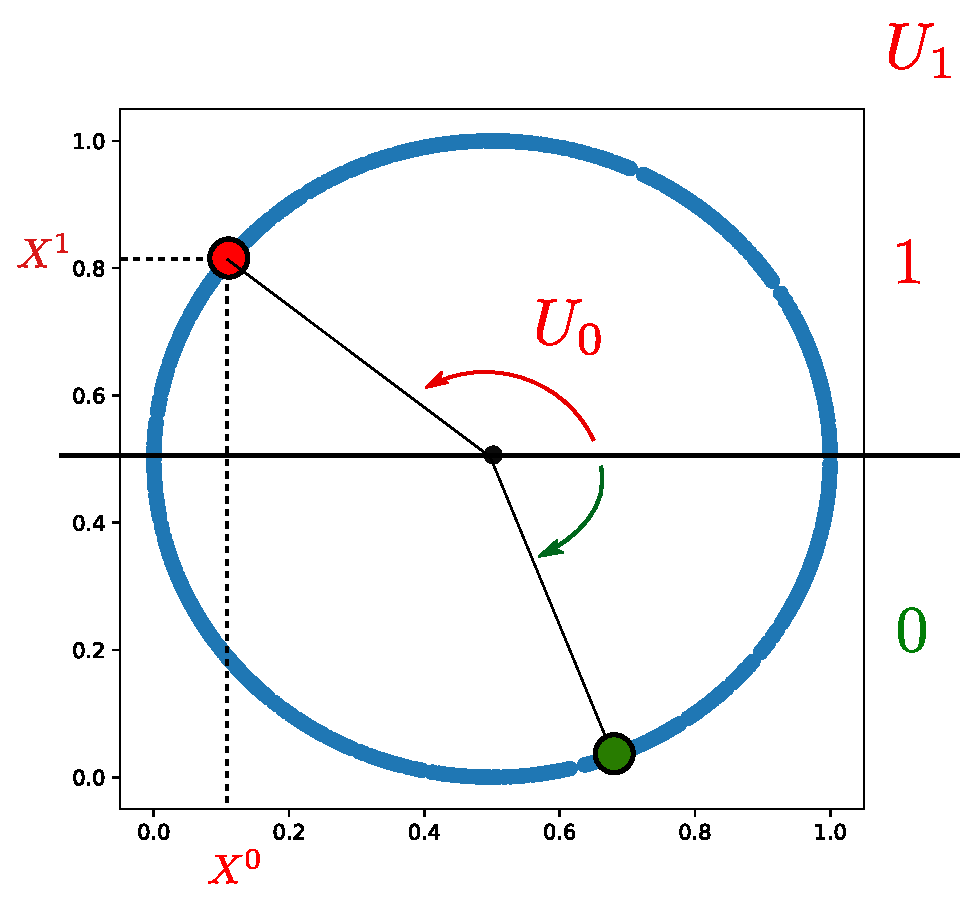
\includegraphics[width=0.6\textwidth]{cercle_2.pdf}
\end{minipage}
\label{fig:U}
\caption{Exemples de paramétrisations du cercle. La paramétrisation qui traduit le plus facilement le modèle est naturellement celle dans laquelle $U$ est à valeurs réelles. Le modèle auxquelles appartiennent les modalités $X^0$ et $X^1$ est donc représenté par la variable cachée $U$.}
\end{figure}

\subsection{Représentation des éléments des cartes}

Le jeu de données d'entrée se décompose en jeu d'apprentissage et jeu de tests. Lors de la phase de test, seul le processus de recherche de la best matching unit est réalisé et les poids des cartes ne sont pas mis à jour. Dans le cadre des variables aléatoires, chaque itération de test est alors un tirage indépendant. Les éléments des cartes peuvent donc être considérés comme des variables aléatoire et une itération de test comme une réalisation de celles-ci. La phase de test peut être réalisée après n'importe quelle itération de l'algorithme d'apprentissage. Le processus d'apprentissage et de tests est décrit en figure~\ref{fig:flowchart}.

Nous considérerons alors plusieurs éléments des cartes en tant que variables aléatoires:  
\begin{itemize}
\item Les positions des BMUs $\bmu\m{0}, \cdots, \bmu\m{N}$ dans chaque carte
\item Les poids externes des BMUs $\w_e\m{0}(\bmu\m{0}), \cdots, \w_e\m{N}(\bmu\m{N})$
\end{itemize}
Tout autre élément d'une carte peut être vu de cette manière, telles que les activités. 
Une phase de test est alors un ensemble de réalisations d'une variable aléatoire jointe : 
$$(\inpx\m{0}, \cdots, \inpx\m{N}, \bmu\m{0}, \cdots, \bmu\m{N}, \w_e\m{0}(\bmu\m{0}), \cdots, \w_e\m{N}(\bmu\m{N}))$$
Les composantes de cette variable jointe ne sont pas indépendantes. Les représentations et indicateurs présentés ensuite chercheront à détecter et comprendre au mieux leurs dépendances statistiques.

Le formalisme par variable aléatoires permet alors d'utiliser des outils et métriques issus de la théorie de l'information pour qualifier l'organisation des cartes au sein de l'architecture.

\begin{figure}
\centering
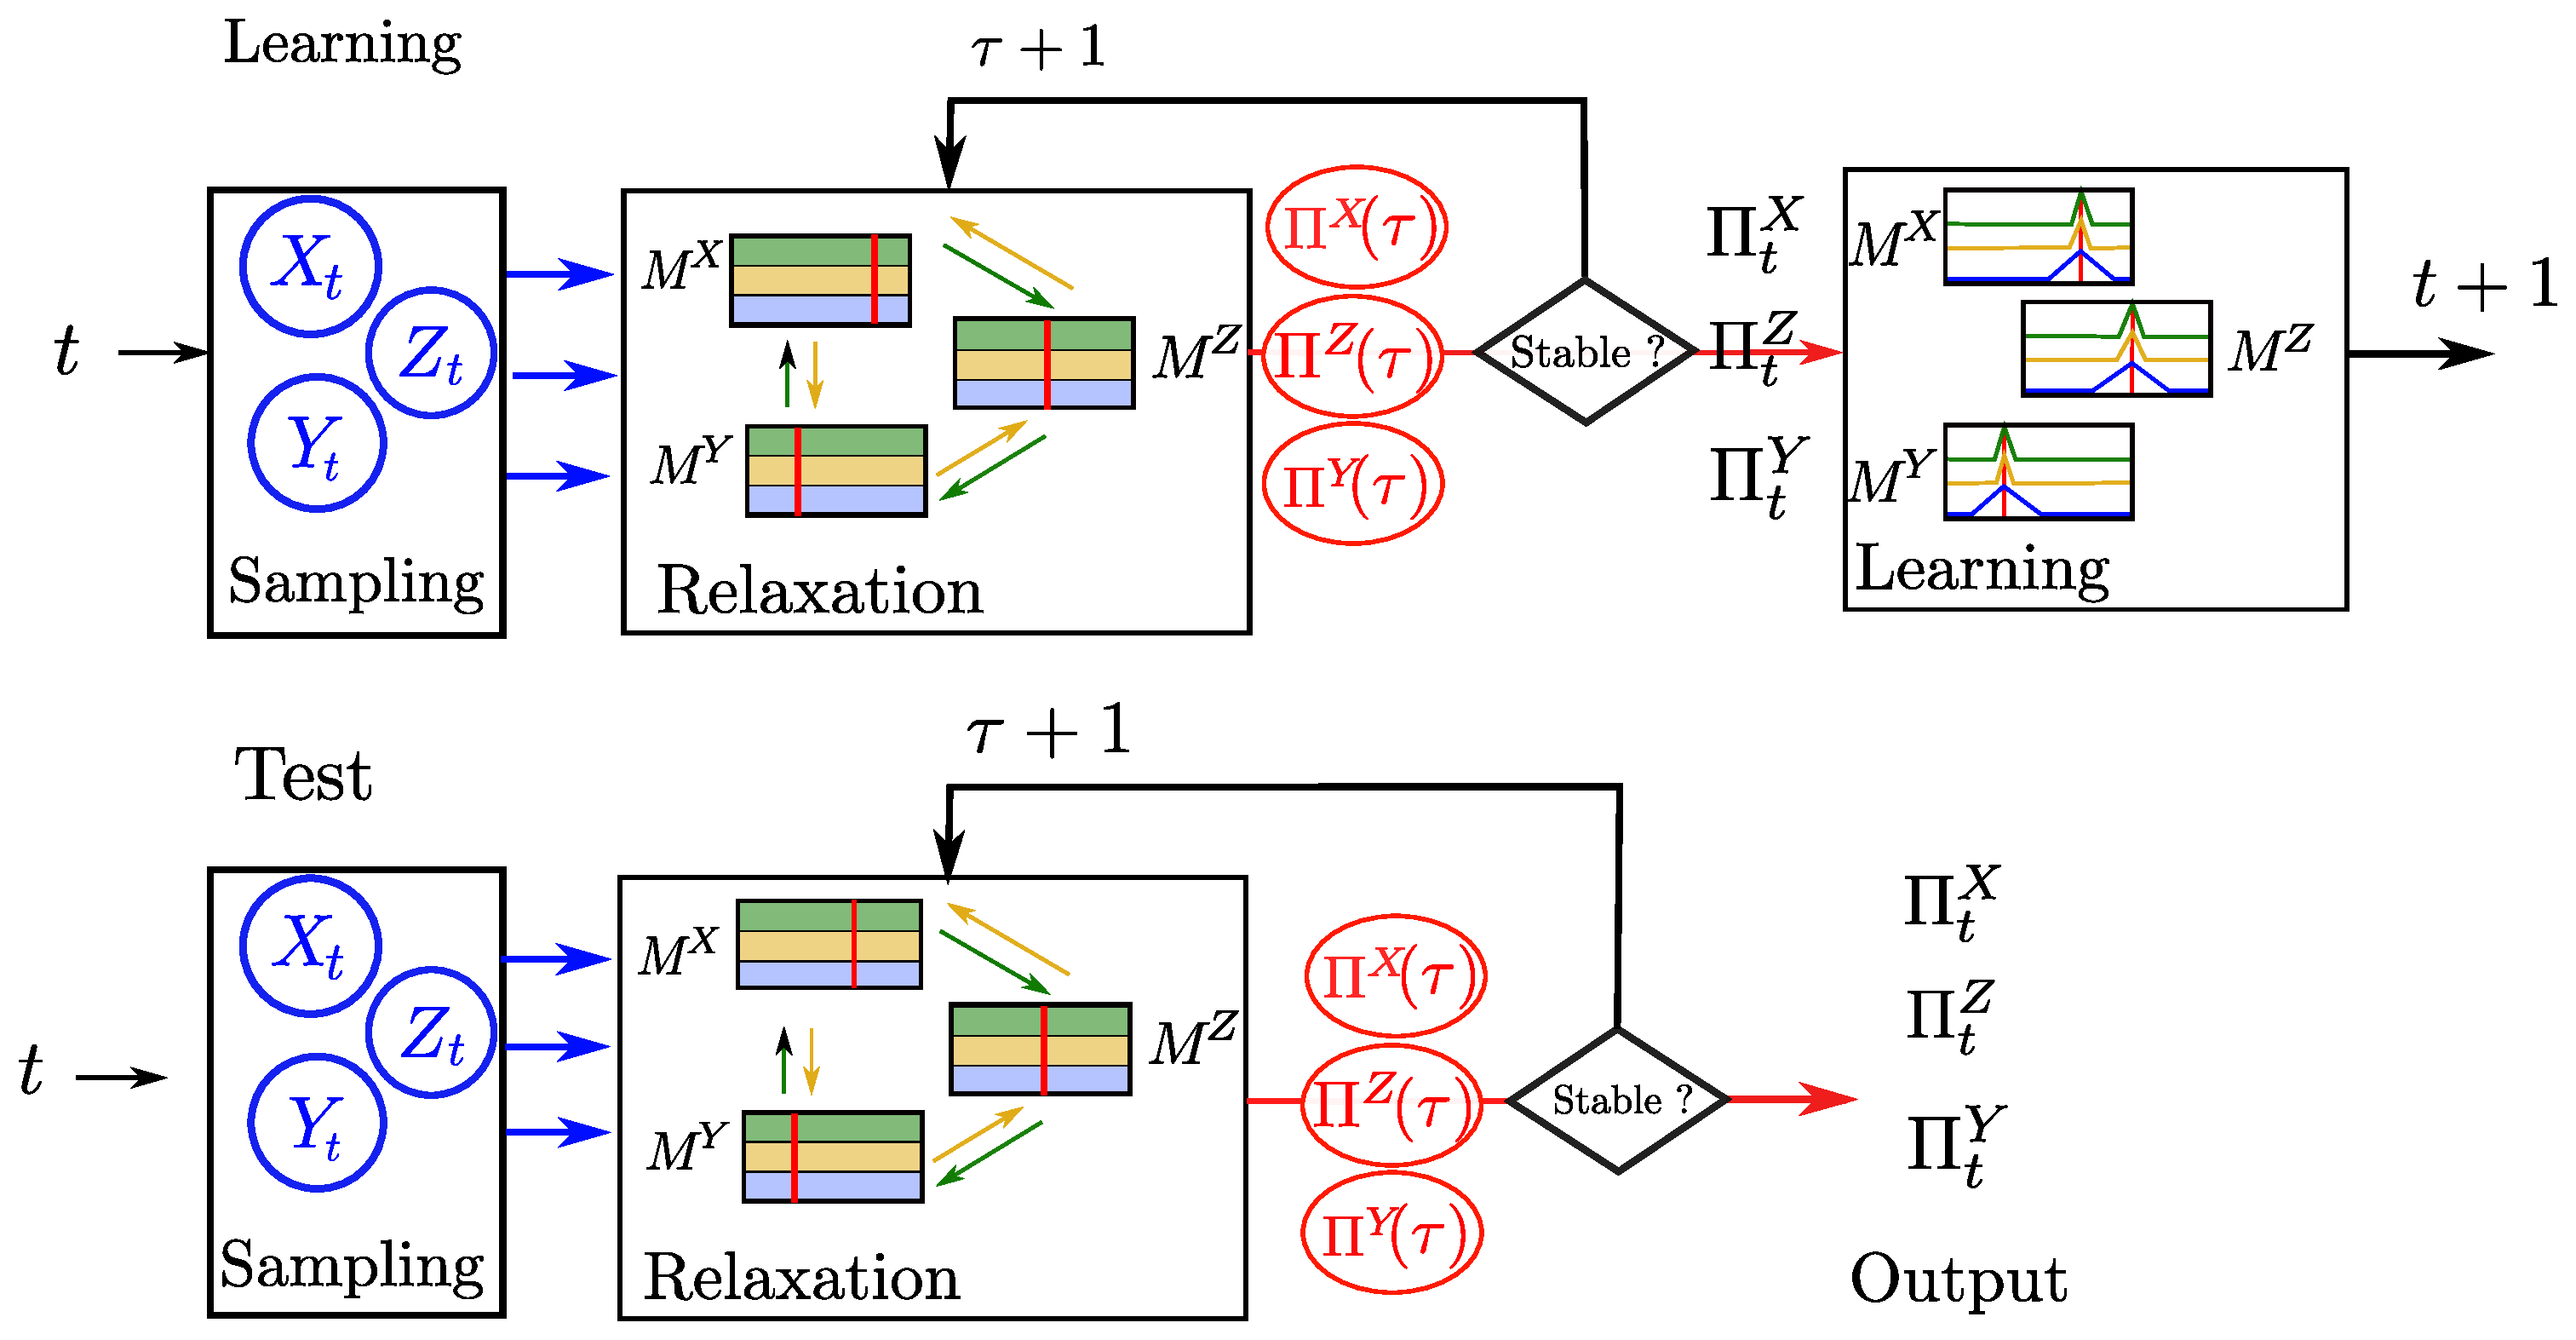
\includegraphics[width=0.7\textwidth]{learning_tests_nopred.pdf}
\caption{Schéma descriptif de l'apprentissage et des tests.}
\label{fig:flowchart}
\end{figure}


\section{Représentations graphiques}

On peut faire le choix de représenter le poids de la best matching unit par rapport à sa position. Cela donne une représentation similaire au tracé du poids de chaque prototype par rapport à sa position dans la carte.  Par contre, cette représentation fera la distinction entre les \emph{unités mortes de la cartes}, c'est à dire les unités qui ne sont jamais best matching unit et qui ne seront donc pas affichées, et les unités qui ont été BMU au moins une fois. Il s'agit d'une représentation qui prend en compte la façon de calculer le BMU.

La question de la répartition des valeurs d'une carte par rapport à la position de leur BMU va plus loin que les poids. On peut représenter, à partir d'un échantillon test, la dépendance de n'importe quelle variable par rapport à la position de la best matching unit correspondante. Nous détaillerons donc dans cette partie les tracés qui nous paraissent pertinents pour la compréhension de l'architecture CxSOM. 

\subsection{Représenter les entrées par rapport à une carte}

En première représentation, nous tracerons la valeur de l' entrée $\inpx\m{i}$ d'une carte par rapport à la position du BMU $\bmu\m{i}$. Cette représentation permet d'analyser la quantification des entrées par la carte. Ces tracés sont réalisables pour des cartes une et deux dimensions, et pour des entrées quelconques, que ce soient des réels ou des entrées de plus grandes dimension comme des images.
Pour mieux comprendre les relations entre entrées et plusieurs cartes, on tracera sur une même figure les entrées de ces cartes selon la position du BMU d'une des cartes.

Le tracé correspondant à l'expérience du cercle est présenté en figure~\ref{fig:inputs}. Représenter les entrées selon les positions des BMUs montre par exemple que lorsque les cartes sont connectées, les deux points rouge et bleu ayant la même valeur de $X$ ont un BMU différent dans la carte $X$, alors que leurs BMU seraient identiques si les cartes étaient indépendante. On peut donc, par cette représentation, associer des entrées à leur BMU. Cette représentation fait apparaître les zones mortes de chaque carte.

\begin{figure}
\begin{minipage}{0.27\textwidth}
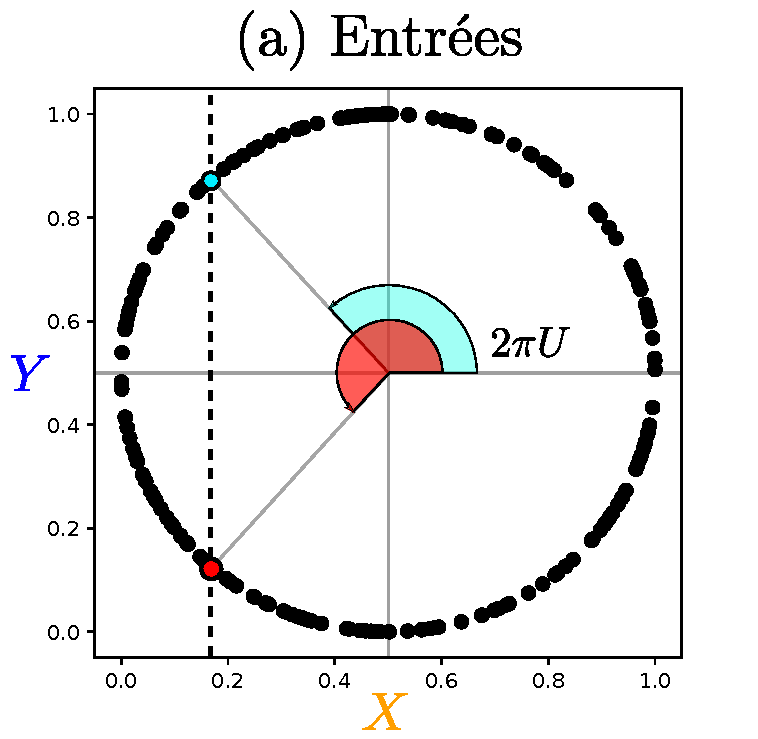
\includegraphics[width=\textwidth]{2som_inp.pdf}
\end{minipage}
\begin{minipage}{0.34\textwidth}
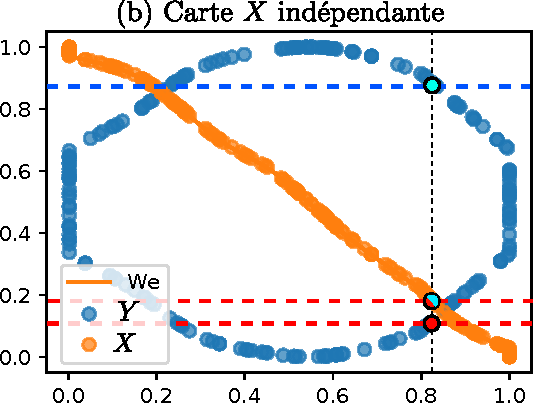
\includegraphics[width=\textwidth]{weights_2som_unco.pdf}
\end{minipage}
\begin{minipage}{0.38\textwidth}
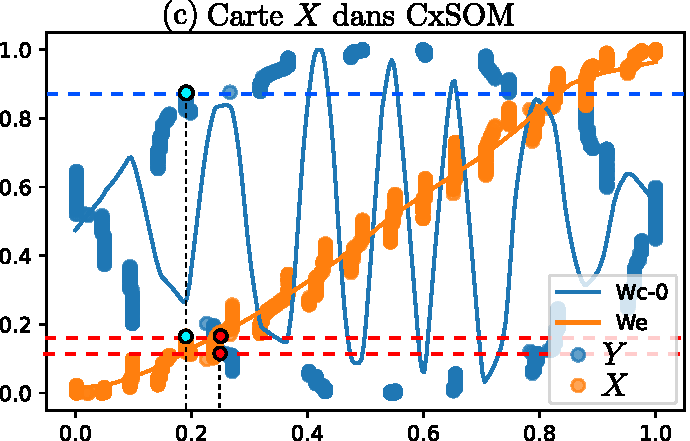
\includegraphics[width=\textwidth]{weights_2som.pdf}
\end{minipage}
\label{fig:inputs}
\caption{Représentation des entrées $X$,$Y$ d'une architecture de deux cartes relativement au BMU de la carte $X$ après apprentissage. Ces tracés mettent en valeur l'organisation des cartes, différentes dans le cas ou les cartes apprennent indépendemment leurs entrées~(b) ou connectées~(c). Les entrées correspondantes sont en figure~(a). Les points bleu et rouge reportés sur les tracés correspondent au même échantillon de test.}
\end{figure}

\subsection{Représentation de U par rapport au BMU}

Pour une, deux, trois entrées, les relations entre entrées se déduisent assez directement. Lorsqu'on augmente la dimension, il paraît pertinent de dégager des nouvelles valeurs qui représentent le modèle: il s'agit ici de la variable $U$. Cette variable cachée est en fait une représentation du modèle en dimension plus faible, par une transformation non linéaire. On peut alors tracer $U$ en fonction de la position $\bmu$ du BMU d'une carte pour représenter comment la position du BMU traduit la relation entre entrées. Le tracé en figure~\ref{fig:piu} montre $U$ comme une fonction de la position du BMU dans chaque carte, contrairement au cas ou les cartes ne sont pas connectées, tracé en figure~\ref{fig:piu_indep}. 

\begin{figure}
\begin{minipage}{0.45\textwidth}
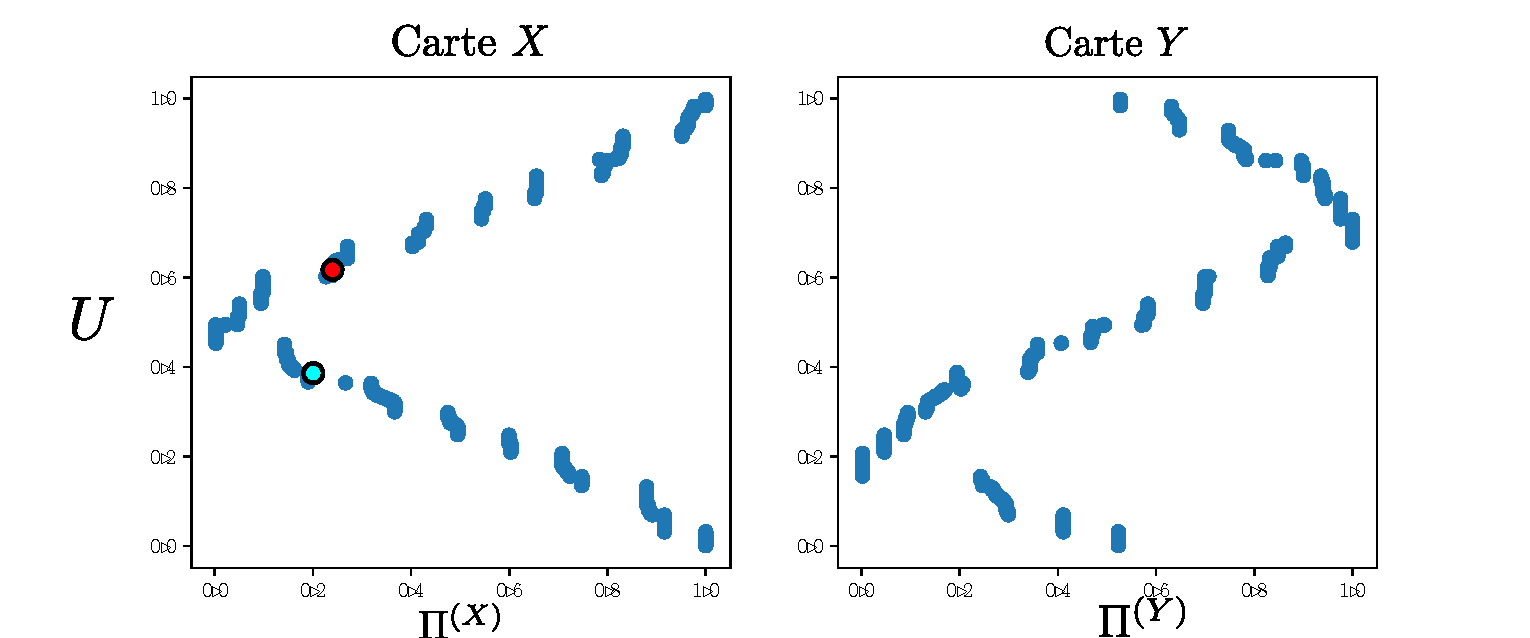
\includegraphics[width = \textwidth]{XU_YU.pdf}
\caption{Valeur de $U$ en fonction des valeurs du BMU $\bmu\m{i}$ dans chacune des cartes, pour des entrées prises sur le cercle. On voit que $U$ est une fonction de la position du BMU dans chaque carte, contrairement au cas ou les cartes apprendraient indépendamment sur les mêmes entrées, voir figure \ref{fig:piu_indep}.}
\label{fig:piu}
\end{minipage}
\hfill
\begin{minipage}{0.45\textwidth}
\centering
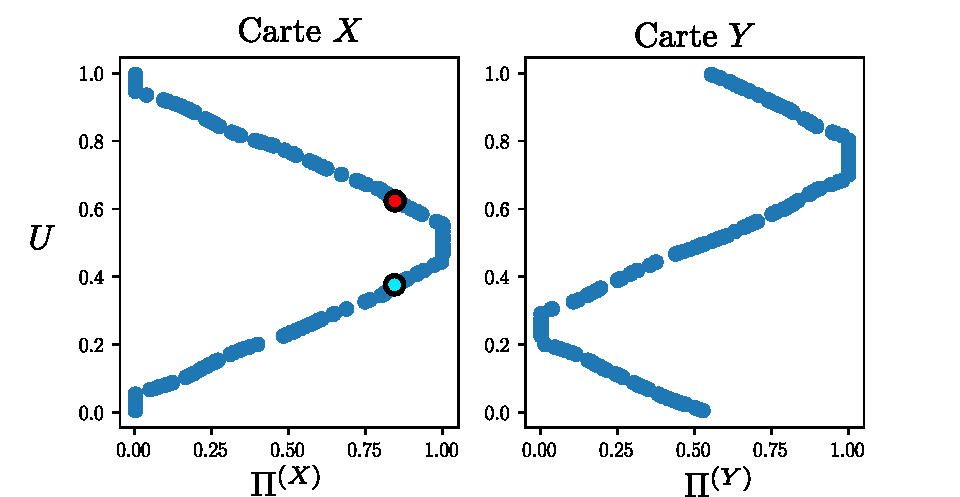
\includegraphics[width = \textwidth]{xu_yu_unco.pdf}
\caption{Pour l'échantillon de test, entrée sur un cercle, valeur de $U$ en fonction des valeurs du BMU $\bmu$ dans chacune des cartes, lorsque les cartes $M\m{X}$ et $M\m{Y}$ ne sont pas connectée. Chacune des cartes n'a aucune information de plus que celle portée par son entrée sur l'état global du système $U$, et $\bmu$ n'est donc pas une fonction de $U$ dans chaque carte. }
\label{fig:piu_indep}
\end{minipage}

\end{figure}


\subsection{Dépliement d'une carte en plusieurs dimensions}

Nous proposons une façon de représenter les poids d'une carte de Kohonen dans l'espace de toutes les entrées. Cette représentation est crée à partir des échantillons de test. Il s'agit de tracer les poids des BMUs dans l'espace de toutes les entrées: $(\w_e(\bmu\m{1}),\cdots,\w_e(\bmu\m{k}))$ dans l'espace en $k$ dimensions correspondant - $k$ correspondant ici à 2 ou 3 dimensions. Les échantillons sont ensuites reliés suivant l'ordre des positions dans \emph{une des cartes}. On obtient ainsi le \emph{dépliement} d'une carte de l'architecture dans l'espace multimodal à plusieurs dimensions. Un exemple de carte ainsi dépliée est présenté en figure~\ref{fig:distortion}.
\begin{figure}
\begin{minipage}{0.5\textwidth}
\centering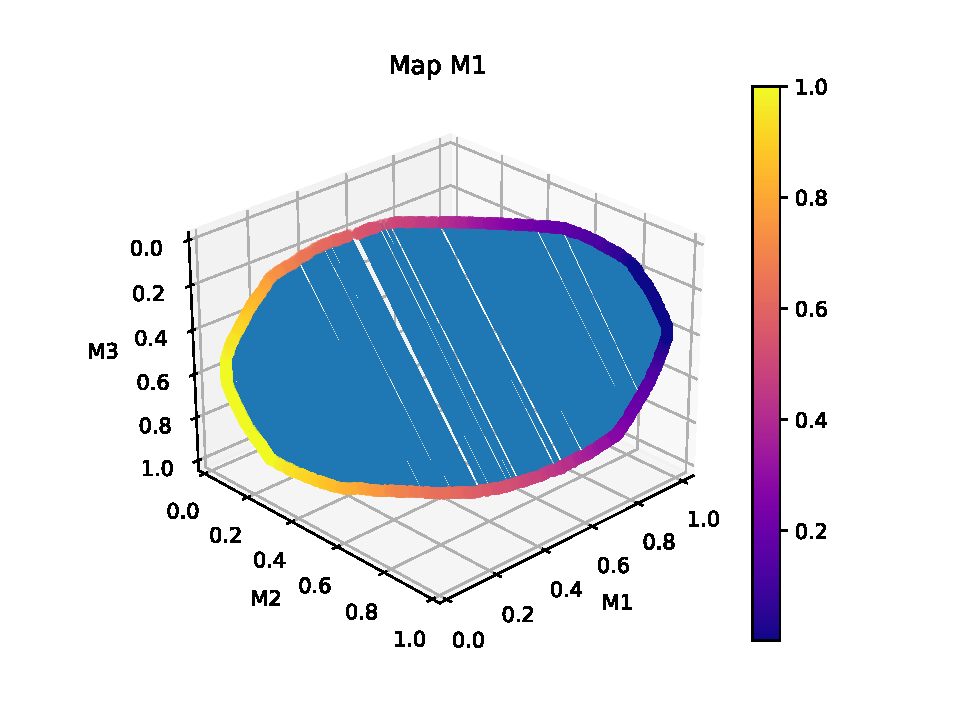
\includegraphics[width=0.8\textwidth]{unco3som}
\end{minipage}
\begin{minipage}{0.5\textwidth}
\centering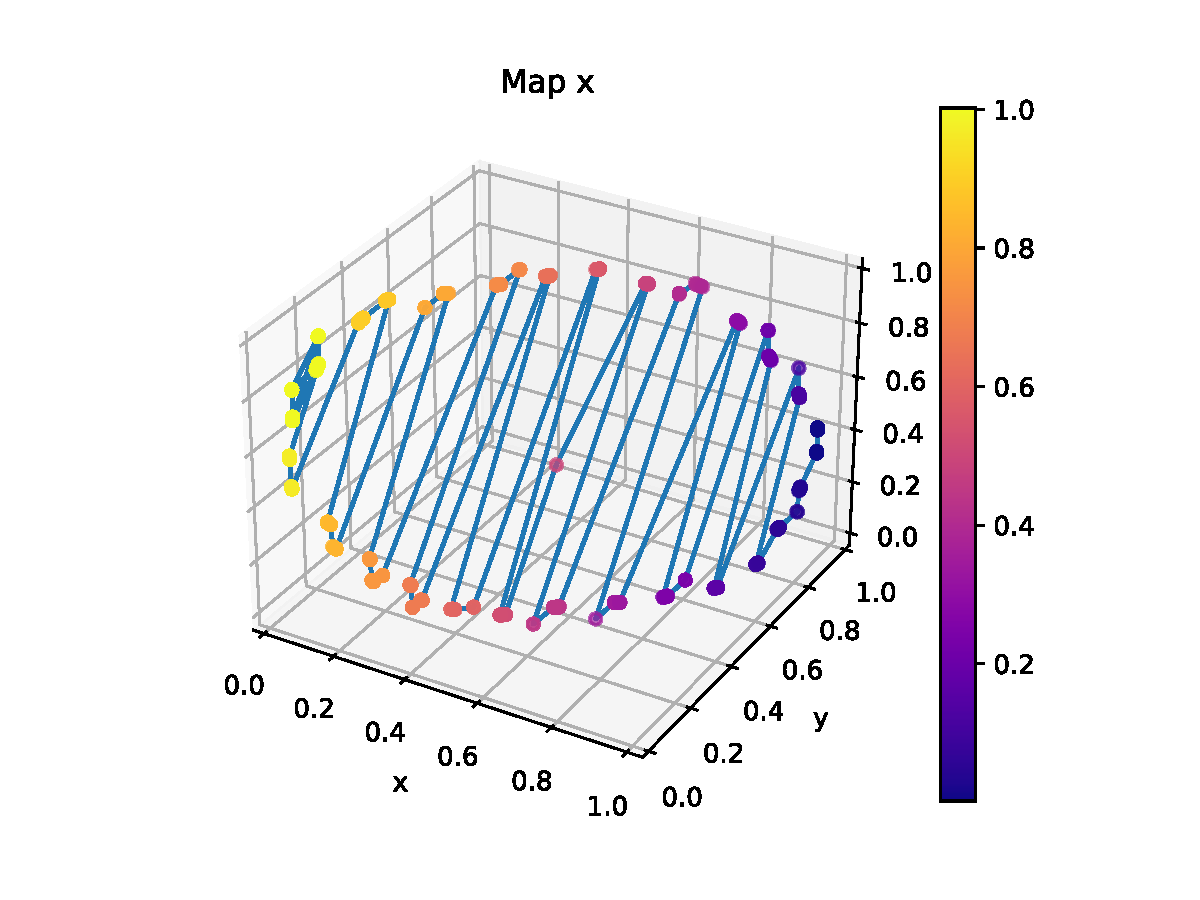
\includegraphics[width=0.8\textwidth]{disto_Mx}
\end{minipage}
\caption{Représentation des poids finaux de trois cartes prenant en entrée $X$,$Y$ et $Z$, reliés selon les positions de la carte $X$. A gauche, les cartes de l'architecture ont appris séparément sur les données. A droite, disposition lorsque les cartes ont été connectées au sein d'une architecture. Un échantillon de 1000 points a été utilisé pour les tracés.}
\label{fig:distortion}
\end{figure}

Ces figures sont équivalentes à tracer une carte dans l'espace de ses entrées: les poids des BMUs de l'échantillon sont les prototypes des cartes; seuls les poids des unités mortes ne sont pas représentés.
Cette représentation est limitée par la dimension des entrées, mais elle peut-être étendue: en plus grande dimension, il est possible de tracer le dépliement de la carte selon un sous-espace choisi de chacune des modalités, ou après réduction de dimension.
Par ailleurs, l'étude du comportement de cartes sur des données 3D s'inscrit dans la démarche de construction d'un modèle que nous suivons dans cette thèse. Leur visualisation est alors un élément clé dans la compréhension des comportements possibles de l'architecture. A partir de cette visualisation, on peut envisager de construire des indicateurs permettant l'analyse de l'architecture en dimension supérieure. 
Le second avantage de ces tracés est qu'il est possible de représenter graphiquement une carte qui ne prend pas d'entrée externe, ou de représenter une carte dans l'espace des poids d'autres cartes.

\section{Information mutuelle comme indicateur statistique}

L'étude de tout processus physique s'effectue par un ensemble signaux issus de capteurs. La théorie de l'information de Shannon \cite{Shannon1948AMT} apporte un modèle mathématique qui abstrait ces signaux et permet de les manipuler, les encoder, les décoder et quantifier l'apport ou perte d'information entre eux, en les utilisant en tant que distributions de probabilités.
Ce modèle mathématique puissant permet de s'abstraire de la nature des signaux pour s'intéresser à leurs relations. Comme son nom l'indique, la théorie de l'information s'appuie sur la notion fondamentale d'information portée par un symbole. Ensuite, cette information se décline en quantités qu'on calcule en fonction de ce qu'on veut mesurer: l'entropie d'une variable, comme l'information apportée par l'observation de la variable seule; l'entropie conditionnelle entre deux variables,l'information mutuelle entre deux variables ou un plus grand nombre. Ces mesures définissent une dépendance statistique générale, et ne dépendent pas du type de modèle ou de relation.

\draft{La théorie de l'information est non seulement applicable, mais en fait profondondément liée aux algorithmes l'apprentissage automatique~\cite{mackay2003information}. L'informatique prend sa source dans les travaux de recherche en la théorie de l'information au XXème siècle. L'apprentissage automatique en est un aspect.
Ces algorithmes cherchent en effet à apprendre un modèle, un signal liant des entrées à des sorties, ou des entrées entre elle. Ce modèle est un encodage du signal d'entrée. 
De son coté, la théorie de l'information apporte un langage fondamental pour quantifier la dépendance entre signaux, les encoder et les décoder. Les algorithmes d'apprentissage étant fondamentalement des encodeurs et des décodeurs, les quantités issues de la théorie de l'information ont donc une traduction directe dans les modèles d'apprentissage, et inversement.
D'ailleurs, de nombreux modèles d'apprentissage automatique se reposent directement sur des règles de calcul d'information pour encoder le signal d'entrée. On pense notamment aux approches bayésiennes de l'apprentissage qui estiment des distributions, et passent par des calculs d'information pour les estimer.}

Nous investiguerons dans cette partie comment quantifier l'apprentissage de l'architecture de cartes par des outils d'information. Bien que cette théorie soit un outil mathématique puissant, il s'agit d'un modèle s'appuyant sur les probabilités. L'estimation à partir de données est donc un élément clé et parfois limitant lorsqu'on cherche à utiliser des valeurs telles que l'entropie pour quantifier l'information au sein d'un système. Nous définirons donc dans cette partie des quantités à mesurer dans l'architecture de cartes, et chercherons à l'estimer.

\subsection{Information mutuelle et entropie}

Les notions d'\emph{entropie} et les valeurs qui en sont dérivées, telle que l'\emph{information mutuelle} entre des distributions, sont des notions fondamentales de la théorie de l'information de Shannon. Ces quantités donnent des informations concernant la distribution d'une variable aléatoire.
Les formules indiquées dans ce paragraphe concernent des variables aléatoire discrètes. 
L'entropie de Shannon d'une variable aléatoire $X$ à valeurs discrètes dans un ensemble $E_X$, de distribution $p(X)$, est notée $H(X)$ et définie par la formule : 
\begin{equation}
H(X) = - \sum_{x \in E_X}{p(x)\textrm{log}(p(x))}
\end{equation}

Elle se mesure en $bit/symbole$ lorsque le logarithme est en base 2, ce qui est généralement utilisé. 
L'entropie est une mesure de la quantité d'incertitude, ou de surprise, sur la valeur de la variable aléatoire $X$. Si la la distribution de probabilité de $X$ est concentrée autour d'un point, l'entropie est faible : lors d'une réalisation de $X$, l'observateur est \emph{plutôt certain} du résultat. En revanche, l'entropie est maximale lorsque lorsque $X$ suit une distribution de probabilité uniforme.
L'entropie s'interpète également comme la quantité moyenne d'information à fournir, en bits, pour coder la valeur que prend la variable $X$.
De la même manière, on peut définir l'entropie conjointe de deux variables, qui est l'entropie de leur distribution jointe, et l'entropie conditionnelle, qui est l'entropie de leurs distributions conditionnelles.

Outre les entropies jointes et conditionnelles, les relations statistques entre deux variables aléatoires $X,Y \in E_X,E_Y$ peuvent être mesurées par \emph{l'information mutuelle}. Elle se définit formellement par : 
\begin{equation}
 I(X,Y) = \sum_{x,y \in E_X,E_Y}{p(x,y)\textrm{log}(\frac{p(x,y)}{p(x)p(y)})}
\end{equation}
Cette valeur mesure la quantité d'information moyenne apportée par une réalisation de $X$ sur la réalisation de $Y$.

L'information mutuelle possède les propriété suivantes:
\begin{enumerate}
\item $I(X,Y) = 0 \Leftrightarrow \textrm{X et Y sont indépendantes}$. L'information mutuelle peut être vue une mesure de la distance entre la distribution jointe de $(X,Y)$, $p(X,Y)$ et la distribution dans laquelle les deux variables sont indépendantes, $p(X)p(Y)$.
\item Elle s'exprime à partir de l'entropie : $I(X,Y) = H(X) + H(Y) - H(X,Y) = H(X) - H(X|Y) = H(Y) - H(Y|X)$
\item Elle est symétrique : $I(X,Y) = I(Y,X)$
\item Pour toute fonction $f$, $I(X,Y) \geq I(X,f(Y)$. L'égalité est atteinte si et seulement si $f$ est \emph{bijective}.
\end{enumerate}


\subsection{Indicateur: coefficient d'incertitude.}

Lors de l'analyse de CxSOM, on s'interroge sur l'information que portent les positions des BMUs $\bmu$ d'une carte sur le modèle d'entrées. Les éléments de la carte ont été définis en terme de variables aléatoire; on peut donc utiliser l'information mutuelle comme une représentation de l'information portée par le BMU d'une carte sur le modèle. Le modèle est représenté par la variable $(X,Y,Z)$, mais aussi par $U$. $I(\bmu, U)$ est alors l'information moyenne que le BMU d'une carte porte sur $U$, donc sur le modèle, et $U$ sur le BMU. On souhaite cependant avoir un indicateur normalisé, qui permettrait, sur une échelle de 0 à 1, de quantifier à quel point un BMU porte de l'information sur $U$. On va donc normaliser l'information mutuelle $I(\bmu,U)$ par la valeur maximale qu'elle peut prendre dans notre carte.


Cette valeur maximale atteinte par $I(\bmu,U)$ est $H(U)$, atteinte lorsque $U$ est fonction de $\bmu$.
En effet, par construction, $\bmu$ est une fonction de $U$ dans une carte de Kohonen: l'algorithme est déterministe et une sortie est définie pour toute valeur de $U$. 
Par propriété de l'information mutuelle, pour toute fonction $f$ et variables $X,Y$, $I(X,f(Y)) \leq I(X,Y) $.
Donc, $I(U,\bmu) \leq I(U,U) = H(U)$
Cette valeur est atteinte si et seulement si $U$ et $\bmu$ sont en bijection, autrement dit, si et seulement si $U$ est aussi une fonction de $\bmu$.


Nous définissons donc un indicateur de la relation entre $U$ et un BMU comme:
\begin{equation}
UC(U|\bmu) = \frac{I(\bmu,U)}{H(U)}
\end{equation}
Ce coefficient n'est pas symétrique, et mesure donc l'information portée par le premier terme sur le second, relativement à la valeur maximale qu'elle peut prendre. Dans le cas des cartes CxSOM, $UC \in [0,1]$. Cette valeur rappelle le \emph{coefficient d'incertitude} entre $U$ et $\Pi$, ou $U$ de Theil \cite{Theil1961EconomicFA}.

%TODO : développer ce point : information portée par plus de variables !
%TODO : calculer et comparer les valeurs pour le cas du cercle.

 
Ce coefficient peut être élargi à plus de variables. On peut ainsi calculer $UC(U | (\bmu\m{1},\bmu\m{2},\bmu\m{3}))$ pour 3 cartes, en considérant la variable jointe $(\bmu\m{1},\bmu\m{2},\bmu\m{3})$. Plus largement, pour prouver qu'on a bien appris un modèle, on souhaite que $UC(U|\bmu\m{1},\cdots,\bmu\m{k})$ soit le plus proche possible de 1.

\comment{Qu'est ce que l'information portée par plusieurs variables représente dans le cas du cercle !}

\subsection{Estimation}
%TODO

\comment{ TODO :
Limitations : biais, variance (definition mathématique ?)
Traduction de ces limitations concrètement, notamment pour le calcul du rapport info/entropie : a quoi doit on faire attention ?
}

\comment{
On veut expliquer comment on s'y prend pour estimer le coefficient d'incertitude. On a plusieurs méthodes possible : estimation par binning et estimations par noyaux, par exemple Kraskov. L'estimation par noyaux est plus précise et limite la variance et le biais de l'estimateur, et sera plus fiable en plus grandes dimensions. ( préciser la source ???)
Si on trace l'évolution de l'info mutuelle pour 2 cartes connectées et non connectée, estimée en binning et Kraskov, on 
}

L'information mutuelle et l'entropie sont des grandeurs probabilistes. Elles sont définies à partir de la distribution des variables aléatoire. Lorsque qu'on ne connait pas les distributions, il est nécessaire d'estimer ces valeurs autrement. 
Une première façon d'estimer l'entropie et l'information mutuelle entre $X$ et $Y$ est d'estimer la distribution des variables $X$,$Y$ et leur distribution jointe $Z = (X,Y)$ en discrétisant l'espace par \emph{binning}, représenté en figure~\ref{fig:binning}. Les variables X et Y sont donc discrétisées en \emph{boîtes} de centres $x_k$ et $y_k$. La distribution de X est alors estimée par: 
$$P(X = x_i) = \frac{n_{xi}}{N} $$, où $n_{xi}$ est le nombre d'échantillons de X tombant dans la boîte de valeur $x_i$ et $N$ le nombre de points. Le même procédé est réalisé pour $Y$ et $Z = (X,Y)$.
L'information mutuelle par binning est calculée à partir de ces distributions discrètes.
\draft{Lorsque la dimension des variables est faible (typiquement 1D), l'estimateur est ?? (fiable ?? comment)}
Des termes de corrections peuvent être apportés. La précision de l'estimation peut être améliorée en choisissant des tailles de boîtes variables. Cependant, lorsque la dimension augmente, le nombre d'échantillon disponibles doit augmenter exponentiellement avec la dimension des variables pour éviter le phénomène de "boîtes vides": à cause de la dispersion des données, de nombreuses boîte $(x_j,y_i)$ ne contiendront pas de points alors qu'elles auraient du en contenir selon leur distribution; l'estimation de la probabilité en ce point sera donc nulle, et l'indicateur faussé. 

Un autre estimateur que le binning est l'estimation par noyaux de Kraskov \cite{2004kraskov}. Cet estimeur passe par une estimation diecte de l'entropie au lieu des densités de probabilités. Le découpage de l'espace se fait en recherchant, pour un couple $(X,Y)$ les k plus proches voisins. Une information mutuelle locale est calculée dans cette zone de l'espace, suivant une formule permettant d'approximer les différences de logarithme par la fonction digamma $\psi$ : 
$$i_j(X,Y) = \psi(k) - \psi(n_{x_j} + 1) - \psi(n_{y_j} +1) + \psi(N)$$
Cette information mutuelle locale est ensuite moyennée sur l'ensemble des points: 
$$\hat{I}(X,Y) = \psi(k) - \langle\psi(n_{x_j} + 1) + \psi(n_{y_j} +1)\rangle + \psi(N)$$
Cet estimateur est meilleur que le binning, car il ?? 
Il permet également d'éviter les boîtes vides du binning, car on n'explorera que l'espace des points. Il semble donc préférable d'utiliser cet estimateur en plus grande dimension.
L'estimation de $UC(X|Y)$ nécessite d'estimer $I(X,Y)$ et $H(Y)$ : leur estimation doit être réalisée dans les mêmes conditions.

L'information mutuelle et l'entropie étant des quantités fondamentales en théorie de l'information, il existe de nombreuses méthodes d'estimations de ces valeurs malgré la difficulté qu'elle pose. On peut notamment citer~\cite{Belghazi2018MutualIN}, qui utilise une approche neuronale pour estimer l'information mutuelle. Ainsi, l'utilisation du coefficient d'incertitude comme indicateur semble réutilisable pour des données de plus grande dimension ou pour plus de cartes, quitte à utiliser des méthode d'estimations plus élaborées. 

\begin{figure}
\begin{minipage}{0.45\textwidth}
\centering
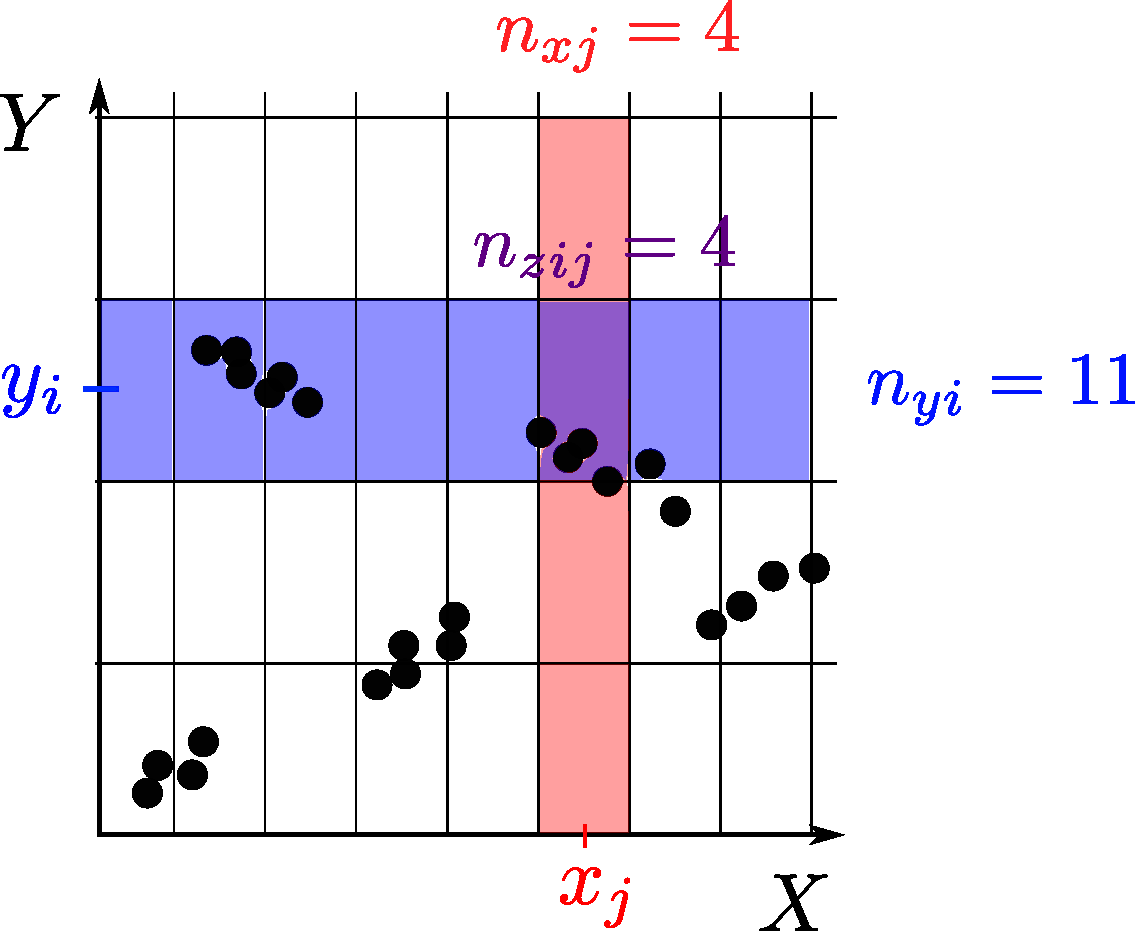
\includegraphics[width=0.9\textwidth]{boxes}
\caption{Procédé de binning pour estimer les distributions des variables $X$ et $Y$. Les distributions sont estimées à partir de $n_{xj}$, $n_{yi}$ et $n_z{ij}$, puis les valeurs de $H$ et $I$ calculées.}
\label{fig:binning} 
\end{minipage}
\hfill
\begin{minipage}{0.45\textwidth}
\centering
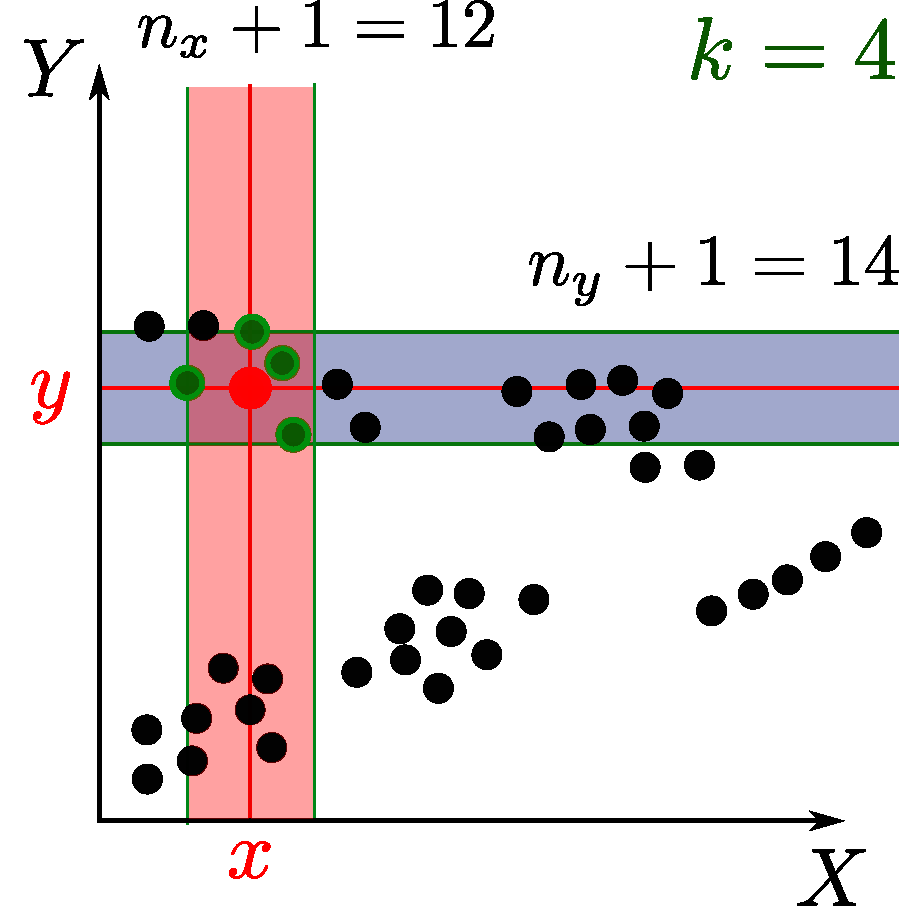
\includegraphics[width=0.7\textwidth]{kraskov}
\caption{Découpage en KNN de Kraskov pour estimer l'entropie et l'information mutuelle des variables $X$ et $Y$. Les plus proches voisins du point rouge sont trouvés, en vert, et le processus est répété sur tous les points. Les valeurs de $n_x$ et $n_y$ permettent d'estimer directement l'entropie.}
\label{fig:kraskov}
\end{minipage}
\end{figure}

%\begin{figure}
%\centering
%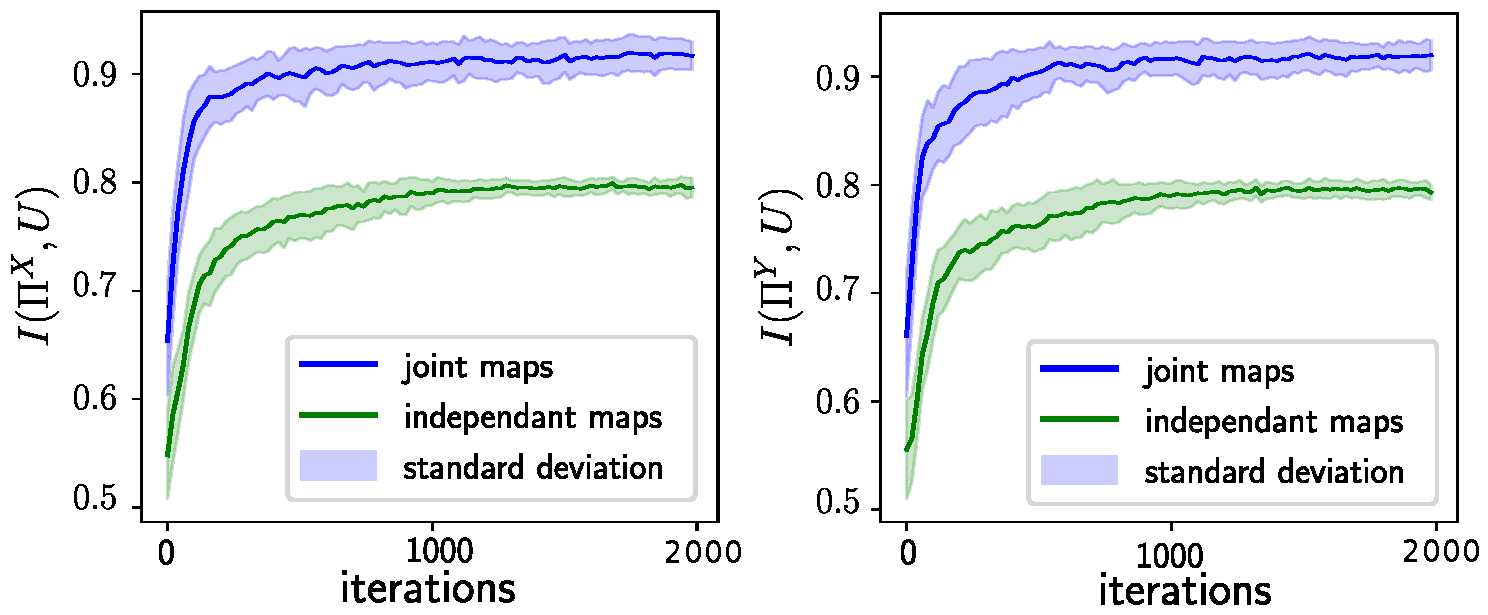
\includegraphics[width=\textwidth]{mutual_info_evol.pdf}
%\caption{Evolution de l'indicateur relatif à l'information mutuelle entre $\Pi$ et $U$ dans chaque carte au cours de l'apprentissage. Cet indicateur est comparé à celui calculé dans le cas ou les cartes apprennent séparément.}
%\label{fig:im} 
%\end{figure}
\draft{
\subsection{Ration de Corrélation}
Un autre indicateur
}

\subsection{Perspectives}

\subsubsection{Erreurs sur les données bruitées}

Le coefficient d'incertitude mesure une forte relation statistique entre les données. Cela mesure bien ce qu'on apprend entre cartes; cependant, il ne prend pas en compte l'aspect continu des variables. Ainsi, prenons une distribution $X$ quelconque et deux distributions $Y_1$ et $Y_2$, telles que représentées en figure~\ref{fig:exemple-limite}.$Y_1$ et $X$ ne sont pas en bijection, mais ont une forte dépendance statistique: lorsqu'on connait la valeur de $X$, seules deux valeurs sont possibles pour $Y_1$.
$Y_2$ et $X$ ne sont pas en bijection, mais en sont proches: leur relation est en fait une bijection, mais avec du bruit. Lorsqu'on analyse des données de CxSOM, les entrées sont généralement bruitées, tout comme les sorties. Par contre, on voudrait privilégier l'existence d'une dépendance forte entre entrées et sorties qui ne tiennent pas compte de ce bruit. Or, dans l'exemple cité, $UC(Y_1|X) = 0.6$ et $UC(Y_2|X) = 0.4$. L'indicateur n'est donc pas complètement approprié dans le cas de variables avec bruit.

\begin{figure}
\centering
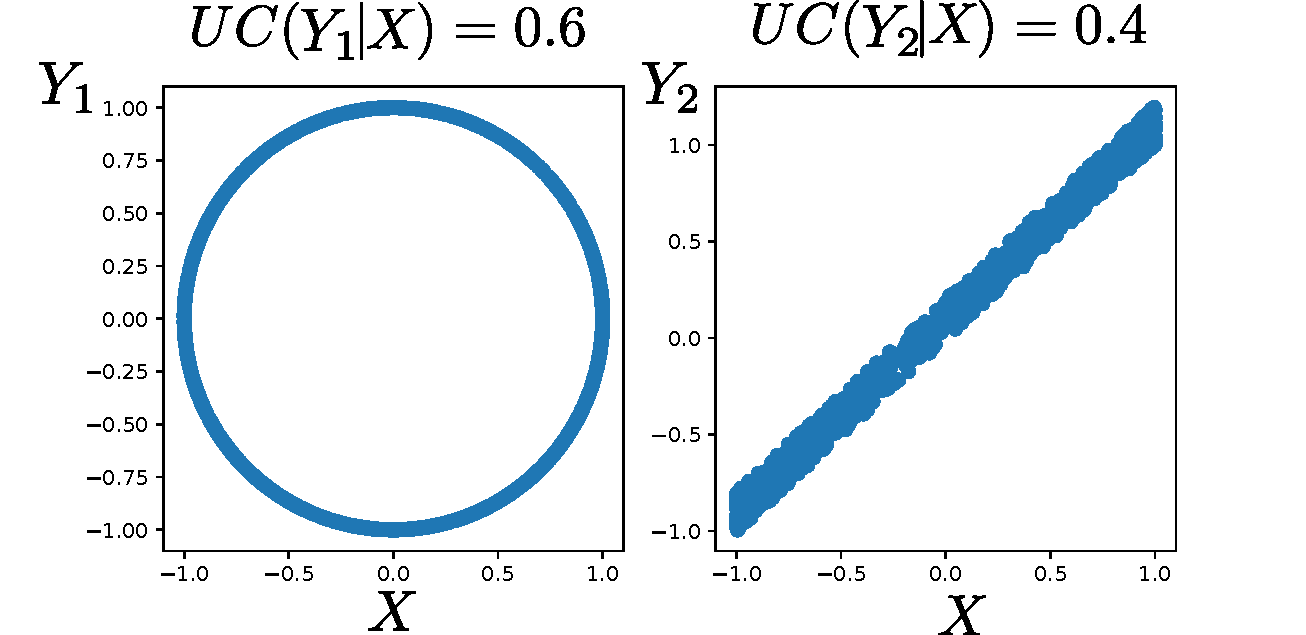
\includegraphics[width=0.7\textwidth]{exemple_limite.pdf}
\caption{Pour ces deux distributions $X$ et $Y$, le coefficient d'incertitude mesure une meilleure dépendance statistique dans le premier cas que le second. On voudrait au contraire privilégier le score de la seconde relation.}
\label{fig:exemple-limite}
\end{figure}

\subsubsection{Perspectives d'amélioration}

\comment{Correlation ration : mesure de dépendance fonctionnelle
Débruitage de l'IM : répétition de l'expérience et moyenne ?}

\subsubsection{Discussion}

Le ration de corrélation traduit mieux que le coefficient d'incertitude la dépendance fonctionnelle entre le modèle et le BMU. Cependant, à l'inverse de l'information mutuelle, une relation non fonctionnelle mais précise (telle que l'exemple du cercle de la figure~\ref{fig:exemple-limite}) entre les variables aura un score très faible. Ce n'est pas non plus voulu. 

Il semble que l'information mutuelle reste le moyen le plus prometteur et le plus général de mesurer la relation entre les éléments des cartes. Dans le cas une dimension, on observe qu'on veut tendre vers U fonction du BMU; on connait mal le comportement recherché en dimension plus grande (cartes 2D, entrées de grande dimension). L'information mutuelle laisse donc l'opportunité à plus d'états d'organisation des cartes de l'architecture d'avoir un bon score. La meilleure perspective serait donc de pouvoir calculer le coefficient d'incertitude sur des échantillons provenant de données non bruitées, ou de pouvoir séparer le bruit des données lors du calcul du coefficient.
Dans cette optique, l'estimateur par binning permet de réduire l'effet du bruit, en choisissant correctement les tailles de boîtes. L'utilisation du binning versus Kraskov reste donc à discuter.
Dans le cas ou le modèle d'entrée est connu, calculer les réponses des cartes sur des jeux de données non bruitées générées artificiellement, après apprentissage sur un jeu de données réelles et bruitée, est une solution. Si le modèle n'est pas connu, des méthodes statistique de réduction de bruit peuvent être imaginées. 

\draft{
\section{Prédiction d'entrée}

Au sein d'une architecture de cartes, il est possible de ne pas présenter à une ou plusieurs cartes de l'architecture leur entrée externe $\inpx\m{i}$. Dans ce cas, une best matching unit peut quand même être calculée par leurs entrées contextuelles. Le poids de cette best matching unit peut alors être vu comme une prédiction de l'entrée manquante. Cette capacité de prédiction peut être à la fois vue comme une application possible de l'architecture, mais aussi comme une façon de représenter \emph{ce que les autre cartes connaissent d'une autre}. Tracer les prédictions d'une carte est donc un indicateur de la façon dont une architecture a appris des relations. 


\comment{
2 parties dans estimation/perspectives : 
d'une part, questionnement sur l'estimation des données bruitées par exemple - pas besoin de proposer des solutions si elles ne sont pas testées ? 
Et parler de l'estimation en grande dimension : ce n'est pas forcément le pb ici. Donc pas la peine...
}
}